\documentclass[12pt]{standalone}
\usepackage{amssymb,latexsym, amsmath,graphics}
\usepackage{amsthm}
\usepackage{setspace}

\doublespacing

\usepackage{pgf}
\usepackage{tikz}
\usetikzlibrary{arrows,automata}
\usetikzlibrary{positioning}

\begin{document}
\pagestyle{empty}
 \centering
 % Main layout borrowed from 
% Author: Yury Chebiryak <http://yury.chebiryak.name/index.html>

 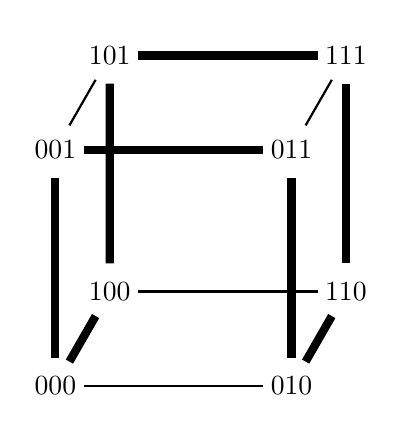
\begin{tikzpicture} [scale=3]
	 \tikzstyle{vertex}=[circle,minimum size=20pt,inner sep=0pt]
	 \tikzstyle{edge} = [draw,thick,-,black]
	 \node[vertex] (v0) at (0,0) {$000$};
	 \node[vertex] (v1) at (0,1) {$001$};
	 \node[vertex] (v2) at (1,0) {$010$};
	 \node[vertex] (v3) at (1,1) {$011$};
	 \node[vertex] (v4) at (0.23, 0.4) {$100$};
	 \node[vertex] (v5) at (0.23,1.4) {$101$};
	 \node[vertex] (v6) at (1.23,0.4) {$110$};
	 \node[vertex] (v7) at (1.23,1.4) {$111$};

	 \draw[edge,line width=3pt] (v0) -- (v1) -- (v3) -- (v2);
	 \draw[edge] (v2) -- (v0);
	 \draw[edge,line width=3pt] (v0) -- (v4) -- (v5);
	 \draw[edge] (v5) -- (v1);
	 \draw[edge,line width=3pt] (v2) -- (v6);
	 \draw[edge,line width=3pt] (v6) -- (v7);
	 \draw[edge] (v7) -- (v3);
	 \draw[edge] (v4) -- (v6);
	 \draw[edge,line width=3pt] (v7) -- (v5);
	 %\node[] at (.66,-.25) {\large $Q_3$};
 \end{tikzpicture}
\end{document}